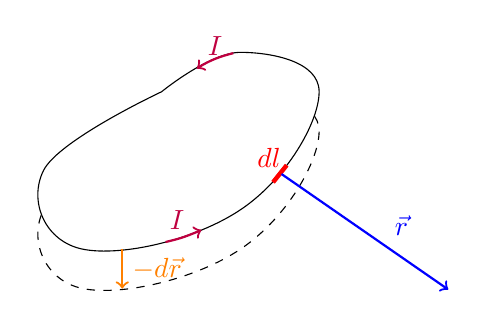
\begin{tikzpicture}
\draw  [dashed]plot[smooth, tension=.7] coordinates {(2,1.5) (0.5,0.5) (1,-0.5) (3,0) (4,1.5) (3,2) (2,1.5)};
\draw [fill=white] plot[smooth, tension=.7] coordinates {(2,2) (0.5,1) (1,0) (3,0.5) (4,2) (3,2.5) (2,2)};

\draw [->, thick, orange] (1.5,0) -- (1.5,-0.5) node [midway, right]{$-d\vec{r}$};
\draw [ultra thick, red] plot[smooth, tension=.7] coordinates {(3.4151,0.85) (3.5884,1.0667)};
\draw [->, thick, purple] plot[smooth, tension=.7] coordinates {(2.0499,0.0916) (2.2666,0.1494) (2.505,0.2433)};
\draw [->, thick, purple] plot[smooth, tension=.7] coordinates {(2.9095,2.4896) (2.7361,2.439) (2.57,2.3668) (2.4472,2.2945)};
\node at (2.6783,2.5762)[purple] {$I$};
\node at (3.3645,1.1609) [red]{$dl$};
\node [purple] at (2.1944,0.365) {$I$};
\draw [->, thick, blue] (3.5234,0.9542) -- (5.6397,-0.5121);
\node [blue] at (5.0474,0.3041) {$\vec{r}$};
\end{tikzpicture}